\textbf{TODO: Incorporate elements of the presentation into the text.} The whole implementation can be found in the GitHub 
\textbf{TODO: Link to repository!} repository. In this section we will show the purposes of each node implementation and how they are related to achieve the desired functionalities.


The implementation timeline was mostly usecase driven since our team did not have any practical experience with the ROS2 middleware and Gazebo Fortress as a simulator. Because of this we decided early on that we need a way to iterate over different implementations and test sensor feedback from the car platform. In order to get familiar with the ROS2 message formats and the implementation of ROS2 nodes in python using \textit{rclpy} as a dependency we implemented the \textit{wasd\_control} node. The node is located in the \textit{test\_package} of our ROS2 workspace. The package is utilized as a point in the project where ideas could be implemented and integrated quickly without interrupting the main stack. The control node acts as a keyboard controller for the ackermann steering system and gave us some insights of how the system needs to be updated in order to get a smooth driving behavior. The node implements a state machine that checks for keyboardThis was also the point in the project where we did face the delays that are introduced by the bad network connection available for the project. We experienced control delays from our machine to the vehicle of up to one second which is infeasible for a live feedback loop. This also limited our capabilities of creating visualizations since we had no way of sending them to our monitors since the network bandwidth was so low.


Because of this limitation and the only local availability of the vehicle we moved to implementing the simulation using Gazebo Fortress. In order to work with Gazebo Fortress we had to familiarize ourselves with the concept of modeling for a simulation and in what file format we want to define our models. Ultimately we chose the SDF file format since it is an open source format with relatively new and comprehensive documentation. The URDF and XACRO formats are mainly associated with ROS in the documentation which introduces a barrier, making it harder to work with. These file formats also separate aspects of the same model into different files. This reduces observability of connected components. Having everything in a single file format also reduces complexity since we only had to learn a single new format. In order to implement the vehicle platform and a world around it we heavily utilized the tutorials on the Gazebo documentation \cite{gazebo-documentation}. The first iteration of the vehicle platform was implemented using their \textit{Build your own robot} tutorial and later remodeled once we had a deeper understanding about the file formats and available plugins. At this stage in the development we were able to utilize the examples implemented in the \textit{gazebo\_tutorials} GitHub repository \cite{gazebo-tutorials}. From the repository we learned how to model the Gazebo UI using SDF files and how to implement the transform tree for our vehicle platform in order to have a better transfer to our ROS2 implementation. In the later stages of developing the simulation we focused on getting the data and structure of the messages as close to the real vehicle platform as possible. This was achieved using the ROS2-Gazebo-Bridge \cite{ros-gz-bridge}. With this bridge we could convert the Gazebo-messages to ROS2 messages and forward the topics to ROS2 as well as remap them to the correct paths if necessary. In the end the simulation was close to interchangeable with the implementation of the car platform and we could reuse our complete software stack in the launch files for Gazebo without heavy modifications.

Due to the theoretical knowledge we obtained from participating in the lecture about autonomous vehicles and artificial intelligence preceding this project our methodology was to implement the best practices we learned in the lecture. This involves a software architecture comprised of different modules that are responsible for subtasks of the overall driving task. The smallest module we could think of was the task of moving to a point in a given coordinate system. In order to achieve that we experimented with the odometry data coming from the drive controller of the simulation and the vesc module of the F1Tenth system stack. We noticed that the coordinate systems between ROS2 and Gazebo are different and started to implement the required logic using the coordinate system from Gazebo with the plan to implement logic to translate it to ROS2. The coordinate system in Gazebo uses the $y$-direction as forward direction and $-x$ as the direction to the right. In this stage of development the \textit{MoveToPoint} ROS2 node. This node receives a new target point using \textit{PoseStamped} messages. Once a target point has been received the node checks its current position using a pose it received from some odometry or SLAM (Simoultaneous Localization And Mapping) topic. From the current pose and the target point it calculates a steering angle using the difference in vehicle rotation and target point direction compared to the current vehicle position. This steering angle is of course clipped by the capabilities of the ackermann steering system but recalculated every time the node receives a new vehicle pose estimation, leading to a smooth steering towards the target point. Once a target point is reached, i.e. the distance to the target point is less than a parametrized $\epsilon$, the vehicle stops until it receives a new target point further away.
Figure \ref{fig:move-to-point} visualizes the calculation of the steering angle using the vehicle orientation and the target point. The red circle visualizes the $\epsilon$ distance below which the vehicle will stop approaching the target point.

\begin{figure}[ht]
\vskip 0.2in
\begin{center}
\centerline{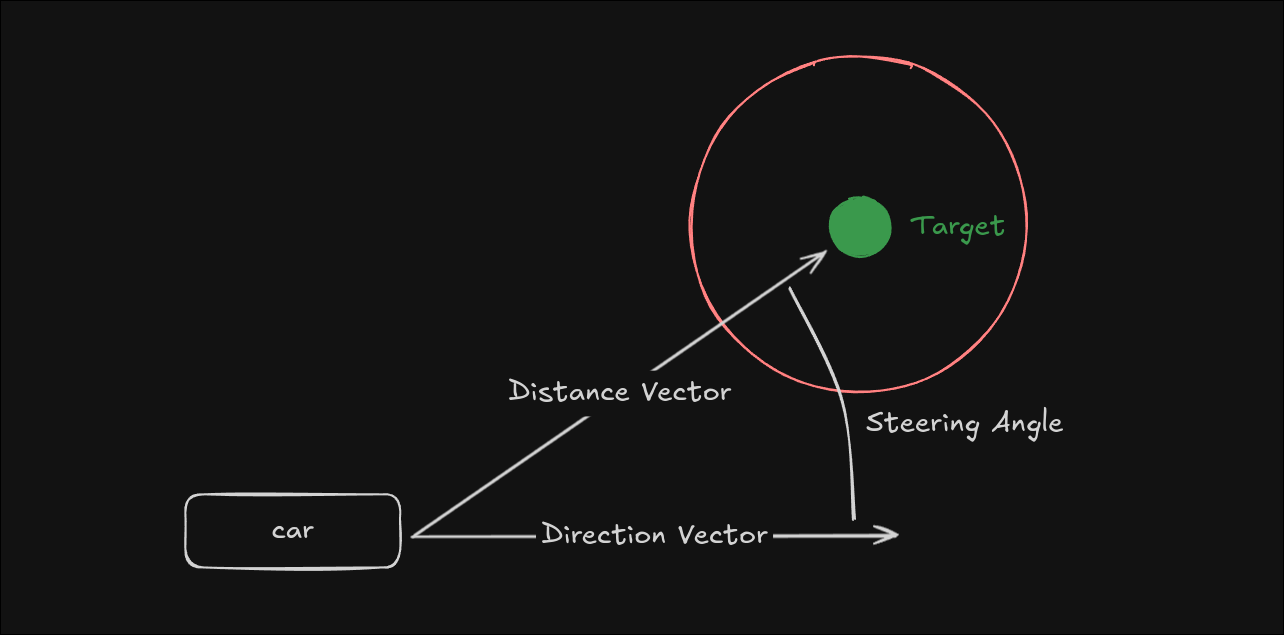
\includegraphics[width=\columnwidth]{move-to-point-vis.png}}
\caption{Schema of the inner workings of the \textit{MoveToPoint} ROS2 node. The figure displays the calculation of the steering angle using vehicle orientation and target point. The red circle marks the $\epsilon$ distance at which the vehicle will stop driving towards the point once inside.}
\label{fig:move-to-point}
\end{center}
\vskip -0.2in
\end{figure}

After iterating over the \textit{MoveToPoint} node we did notice that the coordinate system of ROS2 was in reality more different than expected which we solved using a custom transform at that time. Due to large drifts in the odometry data of the vehicle in the real world we looked into the next building block for our software stack which was SLAM. SLAM would solve the drifting odometry and provide us with the tools necessary to build a map of the environment that we could enhance with additional information from other sensor systems to create a global plan for driving. Implementing SLAM proved infeasible however since during our experiments we noticed that the transforms from the ROS2 transform tree applied to the sensor data used by the SLAM Toolbox yielded very bad results. The sensor data and map information was drifting a lot. The result was an unusable map and no information about even the immediate proximity of the vehicle. Because of this we tried to create a map without using readily available tools like the SLAM Toolbox which also turned out to be infeasible since the noise of the environment requires robust odometry (roboust meaning it drifts in acceptable margins) and elaborate algorithms that could track objects in the environment over multiple frames of sensor data.

\textbf{SEMANTIC MAPPING}

In order to allow control on the platform car we have implemented a \textbf{WASDControl} node that allows manual control of an autonomous vehicle using the WASD keys to send Ackermann steering commands. It listens for keyboard input, translates it into driving commands, and publishes them to the \texttt{/drive} topic.
The \textbf{InitDrive} is responsible for publishing an initial driving command to the \texttt{/drive} topic when it starts. It sends an AckermannDriveStamped message with a predefined speed and no steering angle, while the \textbf{M2P (Move to Point)} node is responsible for navigating the vehicle towards a given target point by processing odometry updates. It listens for target points, calculates the necessary steering and speed, and then sends commands to the \texttt{/drive} topic.\\
\newline
For the cone detection, we have implemented a \textbf{YoloConeDetectionNode} that detects cones in a camera image using a YOLO (You Only Look Once) deep learning model. It processes synchronized RGB images, camera info, and depth images, estimates the 3D positions of detected cones, and publishes the results as DetectedConeArray messages to the \texttt{/yolo\_cones} topic.
The detected cones will be visualized in RViz due to \textbf{ConeMarkerNode} that listens to a DetectedConeArray, transforms the cone positions into a target frame, and publishes visual markers to RViz.\\
\newline
In order to create an occupancy map a \textbf{SemanticGridVisualizerNode} was created that build a semantic map by integrating detected cones into a SLAM-generated occupancy grid. It processes both SLAM maps and detected cones, filters large objects and assigns semantic labels to obstacles.
The \textbf{SemanticGridVisualizerNode} is responsible for visualizing cone clusters detected in a semantic grid using RViz. It processes the semantic occupancy grid, clusters detected cones based on their labels, computes the centroid of each cluster, and publishes visual markers to be displayed in RViz.\\
\newline
Having a map allows us to begin exploring by creating an \textbf{ExplorationNode} that generates target points for an autonomous vehicle by analysing cone positions from the semantic grid. It computes a new driving target point based on the vehicle's position and orientation from the \texttt{/pose} topic, detected cones from the semantic grid, finding the closest blue cone (left) and yellow cone (right) and computing their midpoint as the next driving target. It also monitors steering angle and allows activating/deactivating exploration.
These target points are visualized by the \textbf{ExplorationVisualizerNode} that listens to target point messages and publishes a marker to make the points visible in RViz.\\
\newline
Also for the path planning a \textbf{GlobalPlanningNode} was developed that is responsible for creating an optimized global path for the vehicle to follow after it has completed an exploratory lap. It transitions from exploration mode to global path execution, to ensure that the vehicle follows an optimal trajectory.
